%!TEX root = ../main.tex

\subsection{Batch Algorithm of \ours}
\label{exp:sec:batchalgo}

In Section~\ref{exp:sec:overall} \jks{and Section~\ref{exp:sec:G+},}, $\seven$ \jks{and $\nine$} outperform other baselines on accuracy, but require many human iterations. In this part, we evaluate  the batch algorithm of \ours and \ours$^+ji$ by varying the batch size $b$, \ie Algorithm~\ref{alg:batch} to reduce the number of iterations. Intuitively, the algorithm is  $\seven$  when $b=1$. 
Then we increase $b$ until a single batch with a size $b$ can contain all incomplete tuples in the coreset with size $K$, which is in fact the algorithm $\five$.
 Due to the large number of possible worlds, we adopt the heuristic method in Section~\ref{subsec:batch} to set $l=3$ when $b>1$ \jks{for \ours and we set $l=3$ and $l_G=3$ for \ours$^+$ according to Section~\ref{subsec:pq}}. 

 \begin{figure}   
	\centering
	\begin{minipage}[t]{0.32\textwidth}
		\centering
		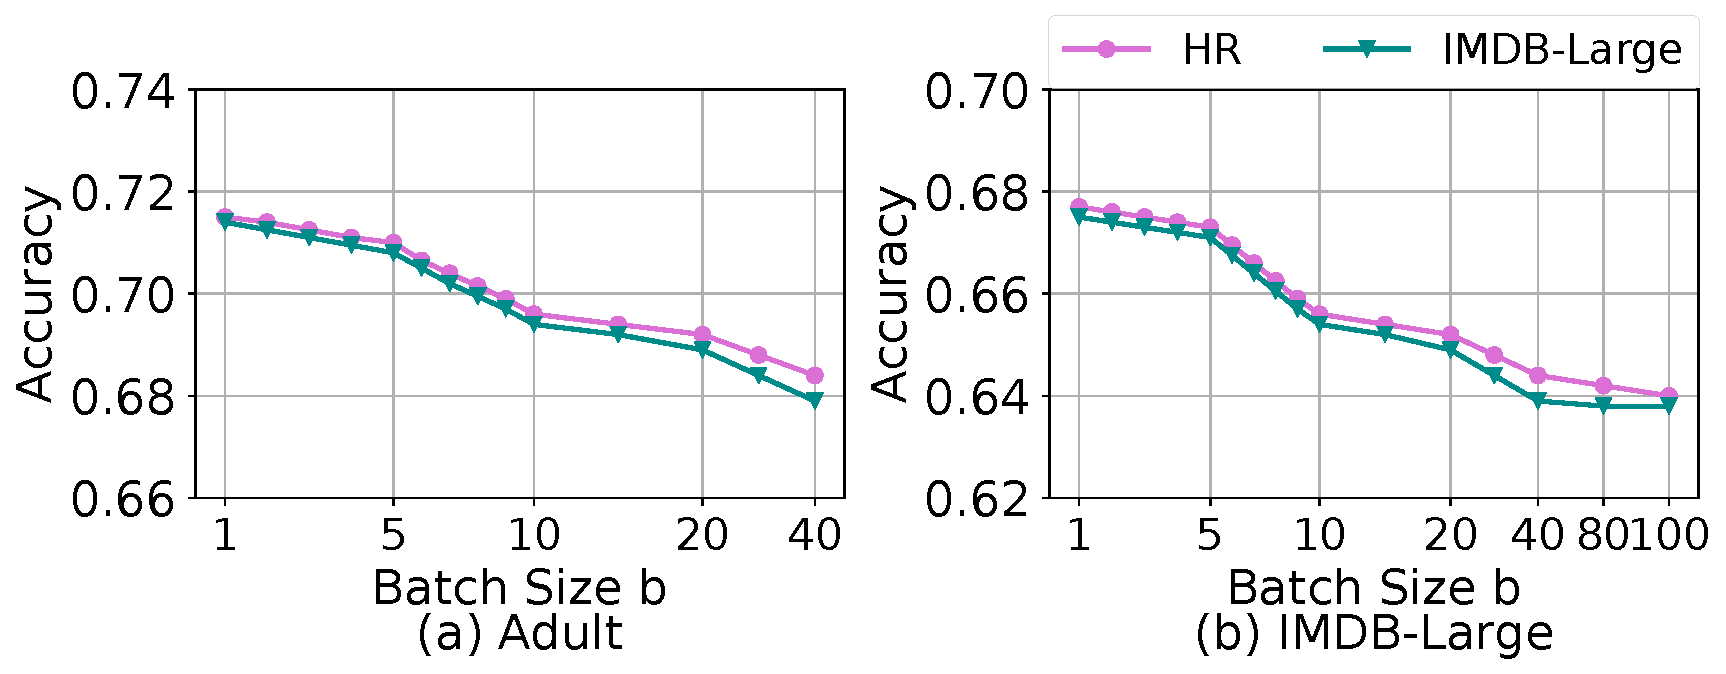
\includegraphics[width=\columnwidth]{figs/batch}
		\vspace{-2.5em}
		\caption{\ours and \ours$^+$ for batch algorithm.}
		\label{fig:batchalg}
	\end{minipage}
	\begin{minipage}[t]{0.32\textwidth}
		\centering
		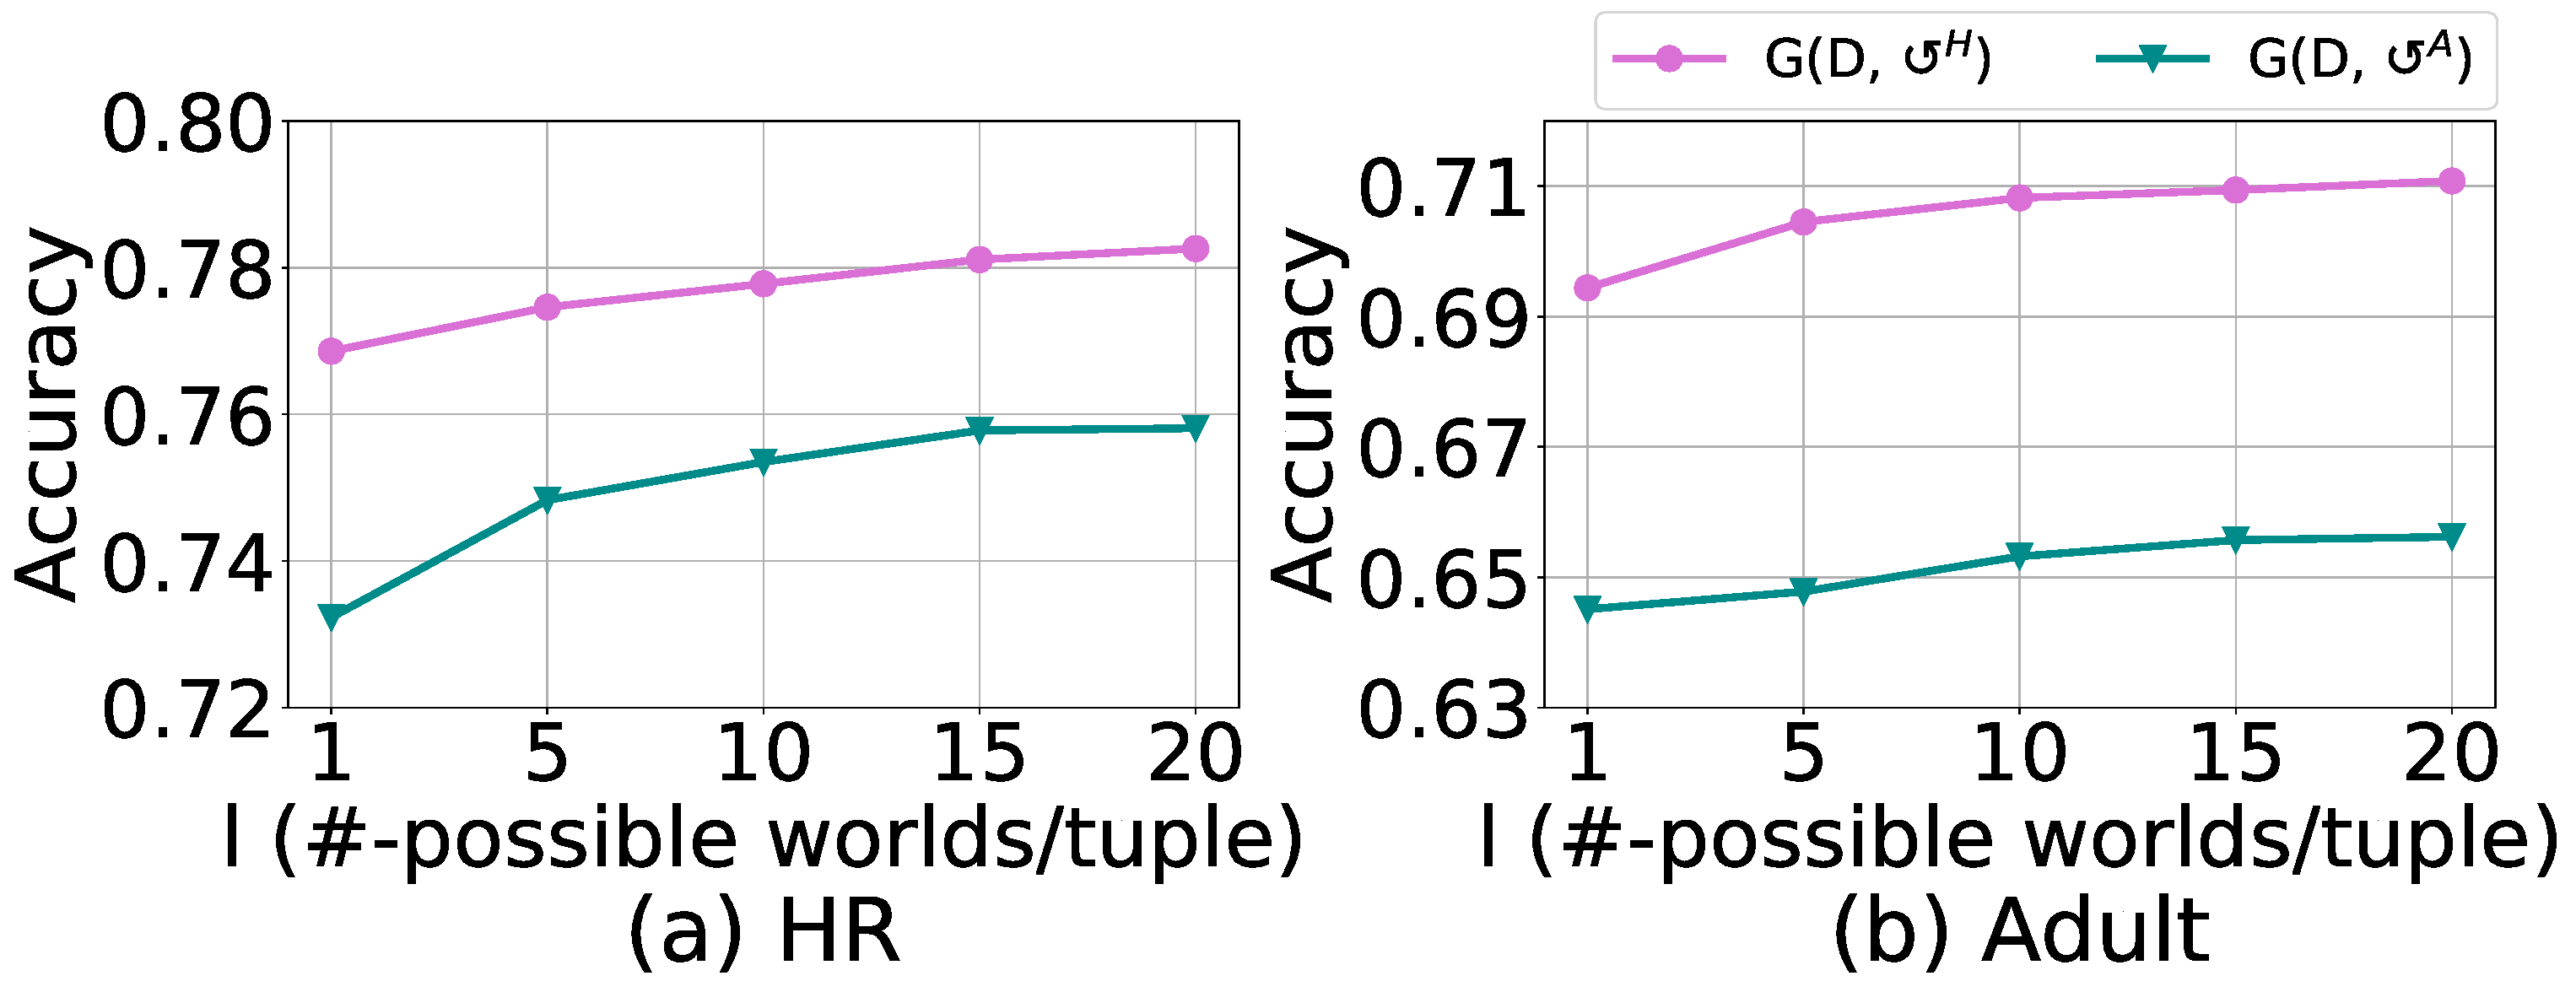
\includegraphics[width=\columnwidth]{figs/vary_l_effectiveness}
		\vspace{-2.5em}
		\caption{Effectiveness of \ours when varying $l$.}
		\label{fig:vary_l_effect}
	\end{minipage}
	\begin{minipage}[t]{0.32\textwidth}
		\centering
		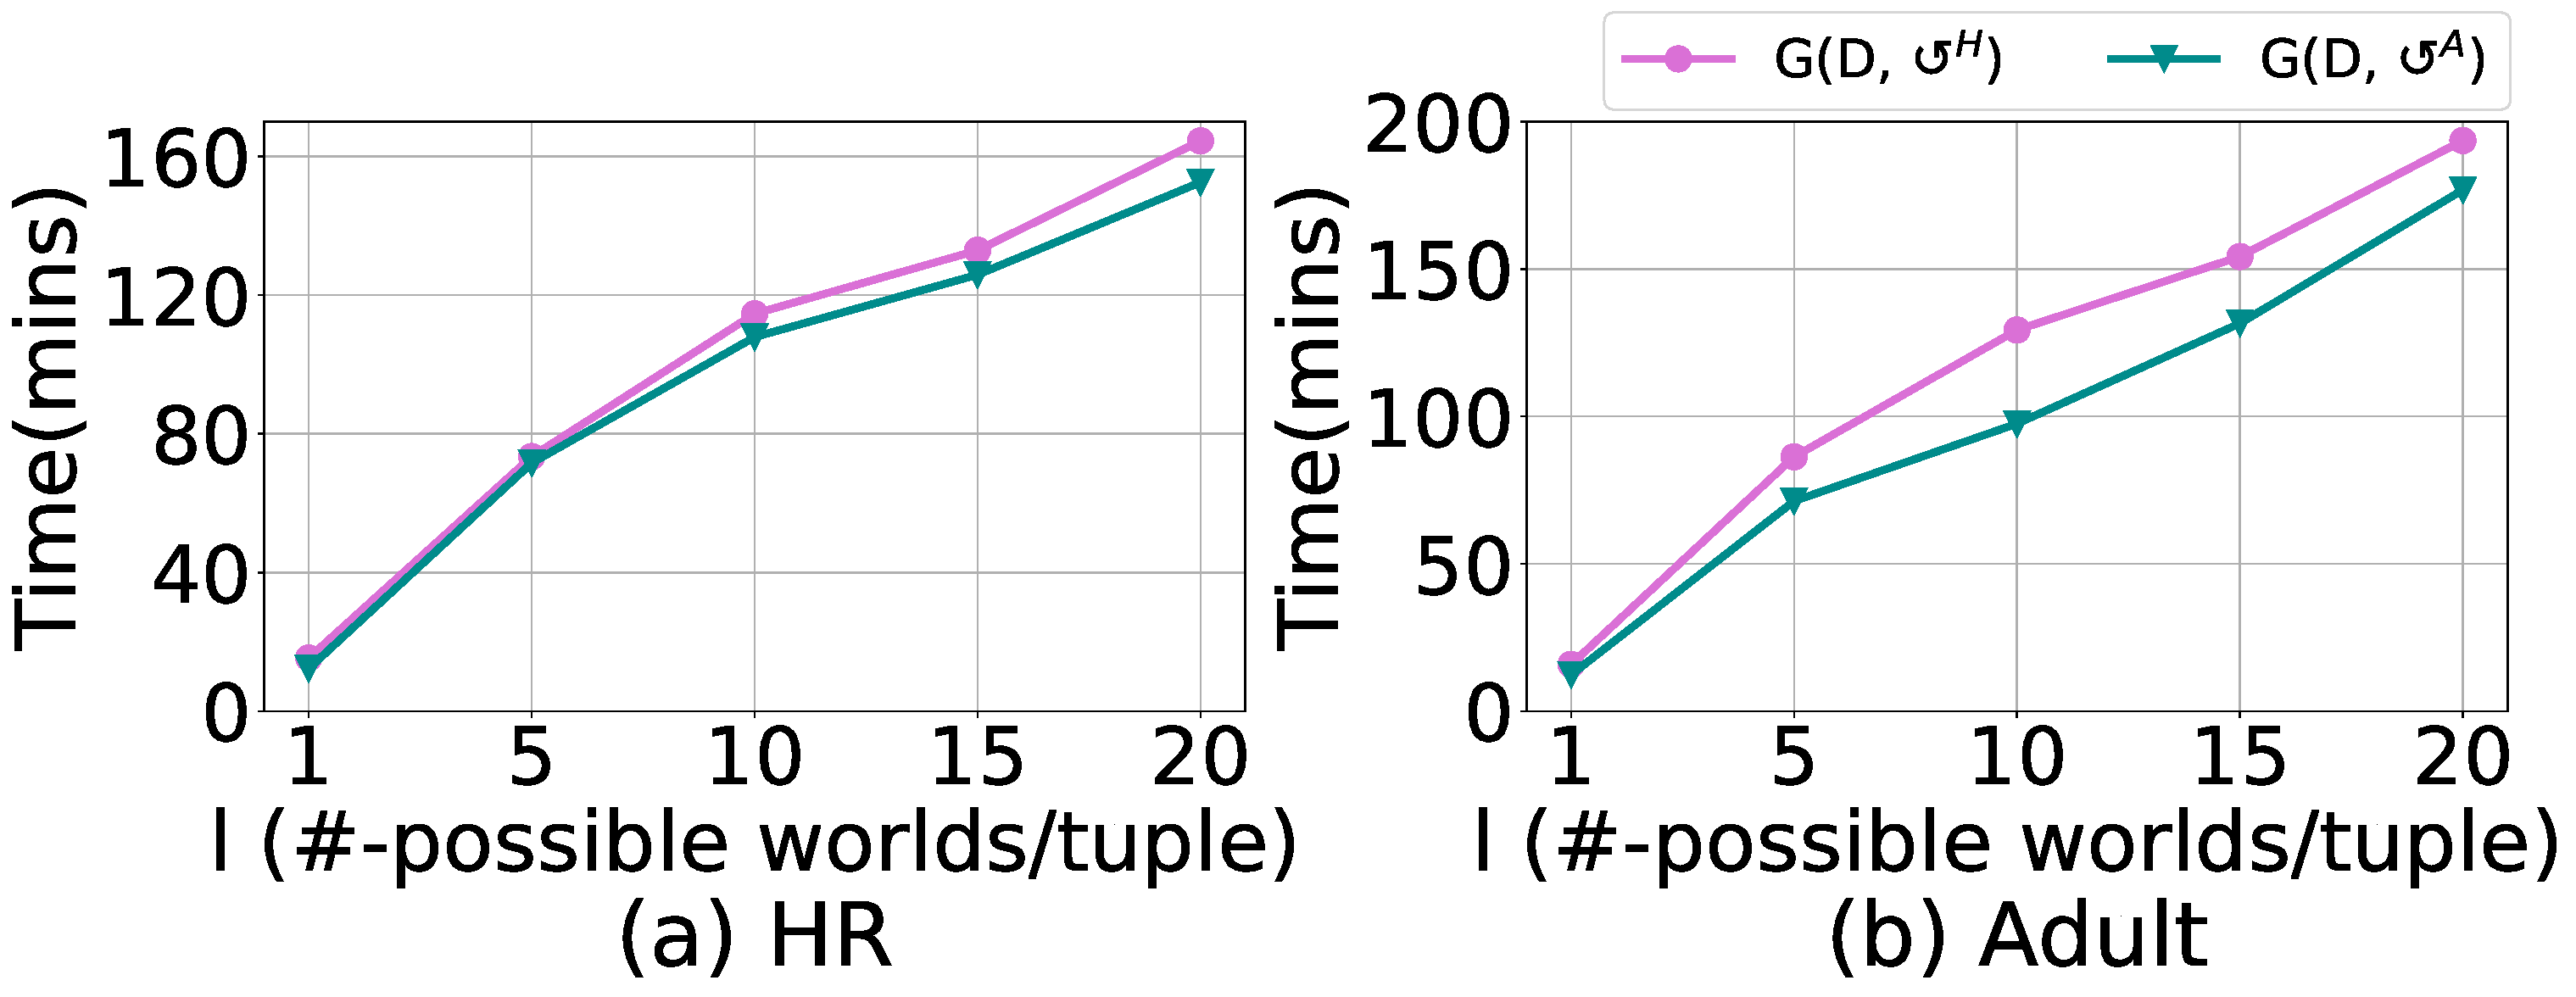
\includegraphics[width=\columnwidth]{figs/vary_l_efficiency}
		\vspace{-2.5em}
		\caption{Efficiency of \ours when varying $l$.}
		\label{fig:vary_l_efficient}
	\end{minipage}
%	\vspace*{-1.8em}   
\end{figure}

% In Figure~\ref{fig:batchalg}, the $x$-axis denotes the batch size and the $y$-axis denotes the test performance on dataset \adult and  \bike. We can see that when $b$ is small (\ie $b \le 5$), the performance does not significantly decrease (\eg on \adult, the accuracy decrease from 71.7\% to 71.2\%.).  When $b$ keeps increasing, the performance slightly decreases. Thus, \ours is not  sensitive to the batch size $b$ and the Algorithm~\ref{alg:batch} can reduce the number of human iterations without sacrificing much  model performance.

\jks{In Figure~\ref{fig:batchalg}, the $x$-axis denotes the batch size and the $y$-axis denotes the test performance on dataset \adult and  \imdbl. We can see that when $b$ is small (\ie $b \le 5$), the performance does not significantly decrease (\eg on \imdbl, the accuracy decrease from 71.5\% to 70.9\% with $seven$.). However, when $b$ keeps increasing, the performance slightly decreases. Thus, \ours  and \ours$^+$ are not sensitive to the batch size $b$ and we can reduce the number of human iterations without sacrificing much  model performance.}


In this part, we also vary the number of possible worlds by varying $l$, which is the number of possibles world per tuple. The larger $l$, the larger number of possible worlds we have. The results are shown in Figures~\ref{fig:vary_l_effect} and  \ref{fig:vary_l_efficient}. In terms of the accuracy, we can see that with $l$ increasing (fixing $b=10$), the accuracy increases first and then  remains stable soon, but the time keeps increasing because more possible worlds indicate more computation. Hence, we do not need a large $l$.

When it comes to the number of possible worlds, we would like to clarify that we do not compare with $\humanfunc(\goodfunc(\train))$ and $\autofunc(\goodfunc(\train))$ because  the number of  possible worlds of $\train$ is very large, which is infeasible to compute. We show the number in Table~\ref{tbl:pwnum}, where we also report the numbers of possible worlds of $\seven$ and $\eight$ in each iteration, which are practical to compute.


\begin{table}
	\centering
	\caption{The number of possible worlds on different datasets}
	{\small
		\begin{tabular}{cccc}
			\hline
			{\bf Method} & {\bf \nursery} & {\bf \hr} & {\bf \adult} \\
			\hline	
			$\five$ & $10^{201}$ & $10^{201}$ & $10^{202}$ \\
			$\six$ & $10^{201}$ & $10^{201}$ & $10^{202}$ \\
			$\seven$ & $10^3$ & $10^3$ & $10^4$ \\
			$\eight$ & $10^3$ & $10^3$ & $10^4$ \\
			\hline
		\end{tabular}
	}
	\label{tbl:pwnum}
	\vspace{-1em}
\end{table}

